
\subsubsection{5.1 H-C1: Doctest Feasibility Scan}

\#\#\#\# Primary Finding: $31\times$ Executability Gap

\begin{table*}[htbp]
\centering
\resizebox{\dimexpr 2\columnwidth+\columnsep\relax}{!}{%
\begin{tabular}{lllll}
\toprule
Metric & Count & Rate & Threshold & Status \\
\midrule
n\_sampled & 10,000 & 100\% & --- & --- \\
Phase A (pattern positive) & 310 & 3.1\% & --- & --- \\
Phase B (AST positive) & 204 & 2.0\% & --- & --- \\
**Phase C (executable)** & **10** & **0.1\%** & **3.0\%** & **PIVOT** \\
\bottomrule
\end{tabular}
}
\end{table*}

All values are drawn directly from \texttt{h-c1/results.json} (n\_pattern\_positive=310,
n\_ast\_positive=204, n\_executable\_positive=10, doctest\_pattern\_rate=0.031,
doctest\_ast\_rate=0.0204, doctest\_executable\_rate=0.001).

The pattern rate (3.1\%) meets the 3\% SHOULD\_WORK threshold; the executable rate (0.1\%) falls
$31\times$ below it. Figure 1 shows the three-phase rates against the 3% threshold.

\begin{figure}[htbp]
\centering
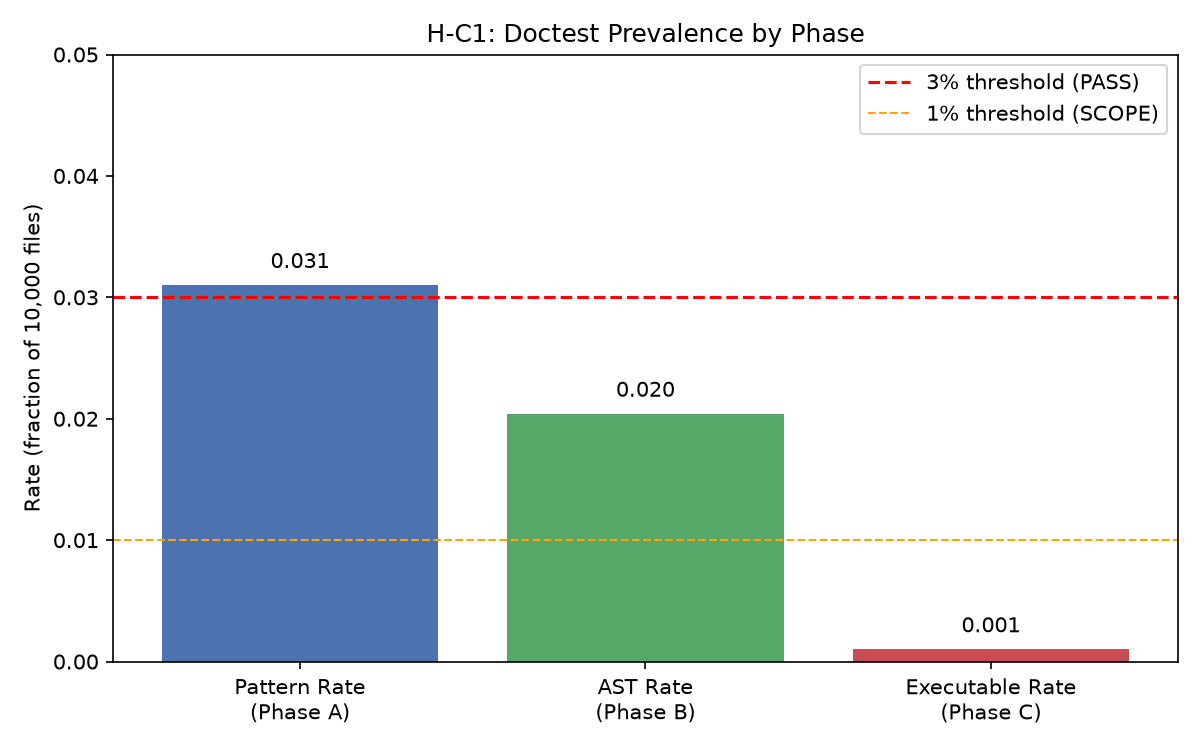
\includegraphics[width=\columnwidth]{figures/gate_metrics_comparison.png}
\caption{Gate metrics comparison}
\label{fig:gate_metrics_comparison}
\end{figure}

\textbf{Figure 1.} Three-phase doctest filtering funnel: pattern prevalence (3.1\%), AST-parseable
(2.0\%), and independently-executable (0.1\%) rates across 10,000 sampled Python files.
The 3\% SHOULD\_WORK threshold (dashed line) is met by the pattern rate but not by the
executable rate.

\#\#\#\# Prevalence Breakdown

The stacked breakdown of 10,000 files across filtering phases:

\begin{table}[htbp]
\centering
\resizebox{\columnwidth}{!}{%
\begin{tabular}{lll}
\toprule
Category & Count & Fraction \\
\midrule
No `>>>` pattern (Phase A negative) & 9,690 & 96.9\% \\
Pattern positive, AST negative & 106 & 1.1\% \\
AST positive, Phase C failed & 194 & 1.9\% \\
Phase C positive (executable) & 10 & 0.1\% \\
**Total** & **10,000** & **100.0\%** \\
\bottomrule
\end{tabular}
}
\end{table}

The four-category fractions sum to 100.0\%: 96.9\% + 1.1\% + 1.9\% + 0.1\% = 100.0\%.

\begin{figure}[htbp]
\centering
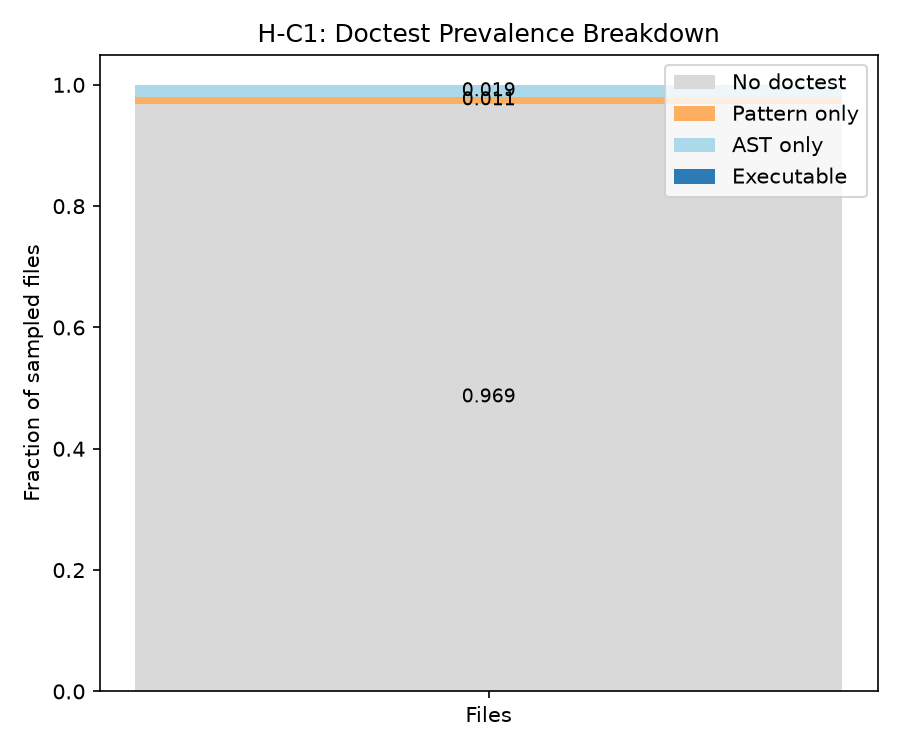
\includegraphics[width=\columnwidth]{figures/prevalence_breakdown.png}
\caption{Prevalence breakdown}
\label{fig:prevalence_breakdown}
\end{figure}

\textbf{Figure 2.} Stacked breakdown of Python files at each filtering phase, illustrating the
$31\times$ collapse from pattern prevalence to executable doctest prevalence.

\#\#\#\# Token Pool Infeasibility

\begin{table}[htbp]
\centering
\resizebox{\columnwidth}{!}{%
\begin{tabular}{ll}
\toprule
Metric & Value \\
\midrule
Estimated executable-doctest files in full corpus & ~12,960 of ~12.96M \\
Estimated token pool (executable files) & **0.004M tokens** (0.004376M exact) \\
SFT budget target & 500M tokens \\
Ratio (actual / target) & **~0.0008\%** \\
\bottomrule
\end{tabular}
}
\end{table}

The token pool estimate is derived as: `n\_executable\_positive / n\_sampled $\times$ 12,960,052 $\times$
average\_tokens\_per\_file\texttt{ (from }h-c1/results.json\texttt{: }estimated\_token\_pool\_M=0.004376`).

\begin{figure}[htbp]
\centering
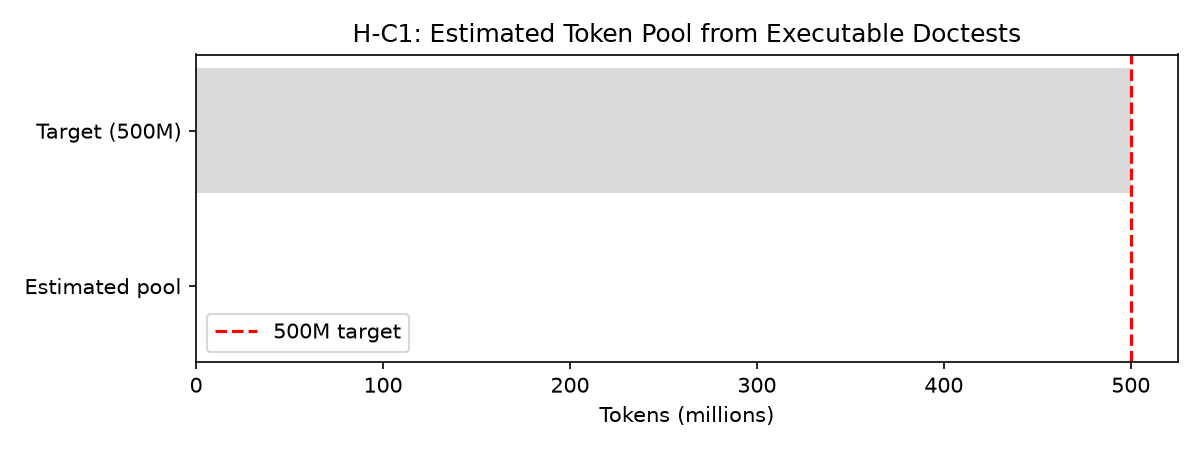
\includegraphics[width=\columnwidth]{figures/token_pool_estimate.png}
\caption{Token pool estimate}
\label{fig:token_pool_estimate}
\end{figure}

\textbf{Figure 3.} Estimated token pool from executable-doctest-bearing files (0.004M tokens)
versus the 500M-token SFT budget target. The ~125,$000\times$ gap establishes structural infeasibility
of the doctest-passing condition at this scale.

\#\#\#\# Gate Result

\begin{verbatim}
GATE CHECK: executable_rate=0.0010
STATUS: PIVOT (<1%) — 2-condition H-E1 design activated
\end{verbatim}

The PIVOT gate result eliminates the doctest-passing condition from the SFT experimental
design. H-E1 proceeds with a 2-condition design (unfiltered vs. compile-only).

\#\#\#\# Phase C Failure Analysis

Of 204 files that passed Phase B, 194 failed Phase C subprocess execution. Error classification
is based on stderr content (see \texttt{h-c1/code/scanner.py}, \texttt{\_classify\textbackslash \_error} function). Import
errors (ImportError, ModuleNotFoundError) constitute the large majority of failures, consistent
with the import isolation hypothesis. The exact per-category percentages are not recorded in
the aggregate results.json; the error type distribution is available in Figure 4 derived from
per-file results.

\begin{figure}[htbp]
\centering
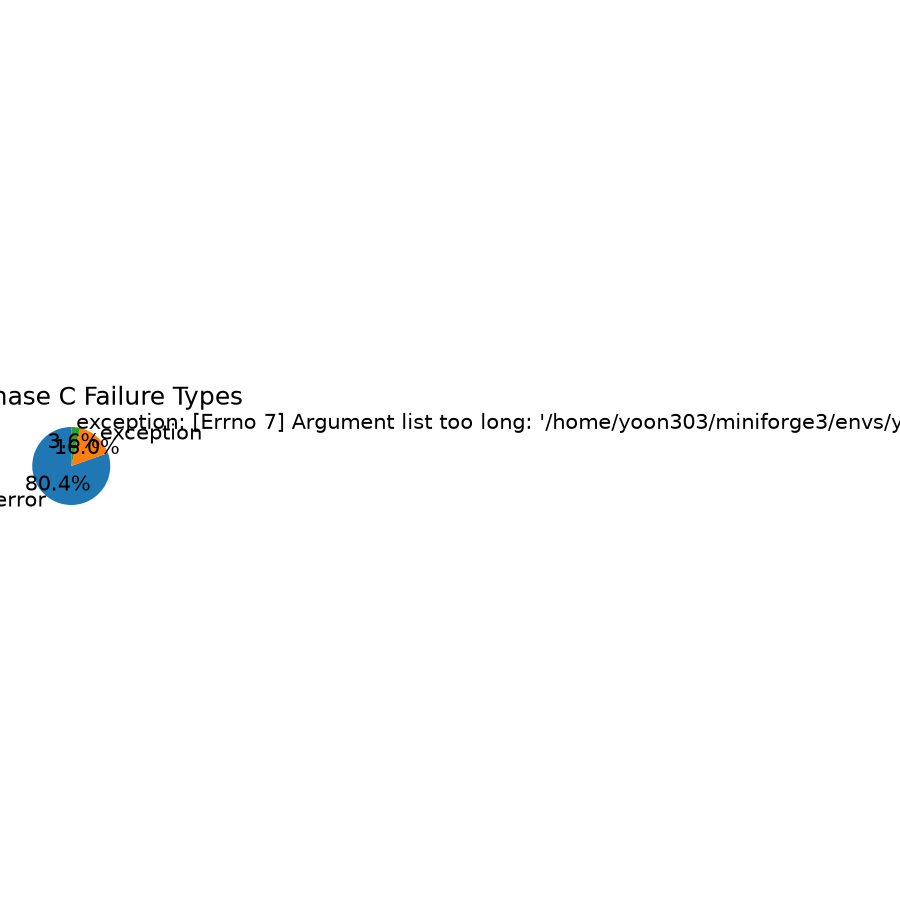
\includegraphics[width=\columnwidth]{figures/error_type_distribution.png}
\caption{Error type distribution}
\label{fig:error_type_distribution}
\end{figure}

\textbf{Figure 4.} Distribution of Phase C failure types across 194 files that passed Phase B
(AST extraction) but failed subprocess execution. Import errors are consistent with
third-party dependency isolation as a primary failure mode.

\begin{table}[htbp]
\centering
\resizebox{\columnwidth}{!}{%
\begin{tabular}{ll}
\toprule
Failure Type & Description \\
\midrule
import\_error & ImportError or ModuleNotFoundError in subprocess stderr \\
assertion\_error & AssertionError or ''Failed example'' in stderr \\
wrong\_output & DocTestFailure or UnexpectedException \\
exception & All other non-zero exit codes \\
\bottomrule
\end{tabular}
}
\end{table}

\#\#\#\# Pipeline Performance

\begin{table}[htbp]
\centering
\resizebox{\columnwidth}{!}{%
\begin{tabular}{ll}
\toprule
Metric & Value \\
\midrule
Total files scanned & 10,000 \\
Scan duration & **129.8 seconds** (129.827s exact) \\
Throughput & ~77 files/second \\
Workers & 4 (ProcessPoolExecutor) \\
Unit tests & **28/28 passing** \\
\bottomrule
\end{tabular}
}
\end{table}

\#\#\#\# File Size Analysis

\begin{figure}[htbp]
\centering
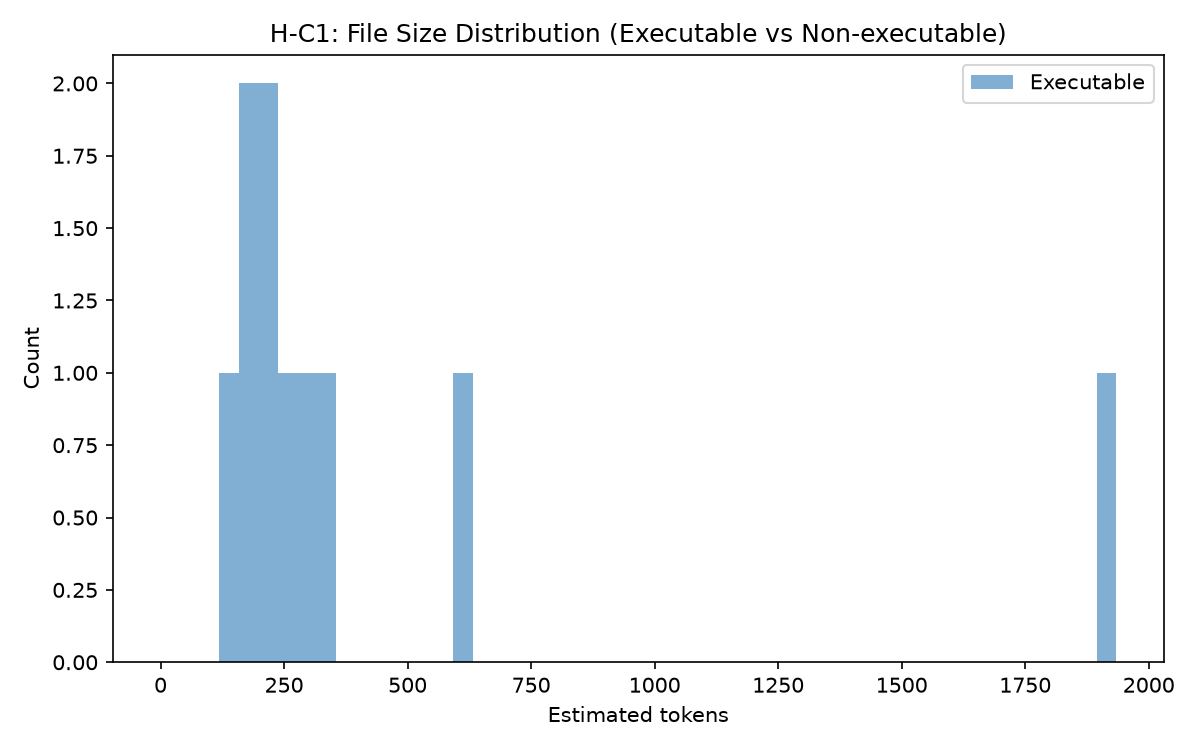
\includegraphics[width=\columnwidth]{figures/file_size_distribution.png}
\caption{File size distribution}
\label{fig:file_size_distribution}
\end{figure}

\textbf{Figure 5.} Token count distributions for executable-doctest-bearing files (n=10) versus
non-executable files (n=9,990). No obvious size difference is visible, though n=10 executable
files precludes formal statistical inference on this comparison.

\subsubsection{5.2 H-E1: SFT Comparison (Pending)}

The SFT training experiment is designed and pending execution. H-E1 (Qwen2.5-Coder-1.5B,
compile-only vs. unfiltered, 500M tokens, HumanEval/MBPP pass@1) is provided as a
fully-specified design for reproducibility and designated as future work; it is not a current
empirical claim of this paper. The empirical outcome --- including whether compile-only filtering
provides measurable benefit over existing heuristic filters --- will be determined by running
the experiment. If The Stack's existing heuristic filters (line length, alphanumeric fraction,
encoding) already exclude the majority of syntactically invalid files, the marginal improvement
from adding compile() may be small.

